\section{Creature and sense details}\label{app:details}

This appendix holds the details moved out of Section 3: how a day and a night work, and how the three senses were built and tested.

\subsection{The creature}

\textbf{Body.} A frozen Qwen3 \cite{yang2025qwen3} base model (Fig.~\ref{fig:1}, top right), 0.6B or 1.7B parameters, served with vLLM \cite{kwon2023vllm} with thinking mode off. Each turn the agent replies in JSON with a short thought, an action and its input, as ``a personal assistant for one user''. The learning adapter (Fig.~\ref{fig:1}, top left) is a LoRA \cite{hu2022lora} of rank 8 on the attention and feed-forward projections of the top 8 layers, loaded into vLLM at run time so each morning's creature uses the previous night's adapter.

\textbf{Day.} In the first step of each day (Fig.~\ref{fig:1}, step 1), the creature works through a fixed number of new tasks (30 a day in every experiment), sampling at temperature 0.7 so it explores. After each attempt the simulated user reacts in words. The true outcome is logged for analysis, but the creature sees it only when the \emph{oracle} is its judge.

\textbf{Night.} At night (Fig.~\ref{fig:1}, step 3) the adapter, and only the adapter, is trained on the lessons with supervised fine-tuning, plus DPO \cite{rafailov2023dpo} ($\beta$ = 0.1) on the preference pairs. Learning rate 1e-4, 2 epochs, at most 40 steps a night. Each night replays the 150 most recent training examples, one per step of a lesson, so old lessons fade out as new ones arrive; on WebShop a lesson takes about 3 or 4 steps, so where each lesson counts once the replay holds about 40--50 lessons, and on $\tau^2$-bench it holds the 150 most recent lessons. A lesson can count once for each of its steps, or once in all, with its loss spread across its steps so that a 15-step attempt counts as much as a 3-step one; Section 4 says which experiments used which.

\textbf{Exams.} The exam (Fig.~\ref{fig:1}, step 4) uses fixed held-out tasks, never learned from, attempted greedily (temperature 0): every morning on WebShop (less often late in the long lives; Section 4), every 3 days on $\tau^2$-bench, and on day 0 before any learning. The next day starts with the adapter that night produced (the loop along the bottom of Fig.~\ref{fig:1}), so each day's work uses everything learned so far.

\subsection{Building the senses}

\textbf{What every version shares.} The sense is a second, frozen Qwen3-0.6B with its own LoRA (rank 16), served beside the creature. Null comes about when the reaction says nothing about the result (silence, ``hmm'', settling, leaving without a word) or when the sense is not confident enough of its answer (under its confidence threshold); v3 adds a third way (below). The sense should commit to a side or abstain, rather than hand the judge a lukewarm 50 to round one way or the other. Each answer begins with a different token (0, 2, 8, 1, n), so the sense decides in one forward pass, and its confidence is the probability of that first token.

\textbf{Sense v1: one dataset's labels.} The first version learned without a teacher, from 45,514 reactions: 39,775 from WildFB \cite{peng2026wildreward}, whose own four-level satisfaction labels we mapped to 0, 20, 80 and 100 (rejection, correction, positive engagement, thanks or praise), and 5,739 silent or non-committal replies we added as null. It reads with a fixed confidence threshold of 0.70 instead of a calibrated one. On held-out WildFB reactions it gave a verdict on 66\%, 94\% of them on the right side, with 2.9\% false accepts. Its weakness shows on the reactions of Table~\ref{tab:4}: it took warm thanks for a failed attempt (``Thank you so much for trying! I'll look on my own'') and a lukewarm ``I guess that'll do'' for full praise, both with confidence above 0.9. One dataset's labels hold few such hard cases (politely unhappy, settling, sarcastic), and v2 set out to cover them.

\textbf{Sense v2: a teacher.} We built v2 by distillation \cite{hinton2015distilling}, from conversations unrelated to our tests. Its raw material is 110,906 moments from six public datasets where an assistant delivered something and the user's next turn shows how they took it: WildFB \cite{peng2026wildreward} and WildFeedback \cite{shi2026wildfeedback} (30,000 each, both drawn from WildChat \cite{zhao2024wildchat}), Taskmaster 1-3 \cite{byrne2019taskmaster} (20,000), MultiWOZ 2.2 \cite{zang2020multiwoz} and ReDial \cite{li2018redial} (15,000 each) and CCPE-M \cite{radlinski2019ccpe} (906; Table~\ref{tab:A3}). Turns where the assistant only asked a question were skipped, since the answer is not a reaction, and shopping was left out, since it is the test domain. Real data rarely holds the hard cases, so the teacher also wrote 4,728 reactions of eight kinds (politely unhappy, settling, vague, sarcastic, ``not my style'', firm rejection, building on the result, plain acceptance) across ten task types and six personas, chosen to differ from our WebShop user's.

A teacher, Qwen3-32B, labelled every reaction under a written guide. It saw the assistant's reply as context; the student never does. Instead of one label we kept the teacher's probabilities over the five answers, read from the log-probabilities of its first answer token, so the student learns the teacher's doubt as well as its choice. On the two datasets that carry their own signal of success, the teacher agreed with it on yes or no 81\% (WildFB) and 85\% (WildFeedback) of the time, and it called about half of the WildFB reactions unclear. The student inherits the teacher's mistakes as well as its knowledge; the confidence threshold below is meant to keep them out of the creature's lessons.

The student learns to match the teacher's probabilities (KL divergence) on 47,800 reactions, balanced so that no task type or answer dominates, for one epoch (learning rate 1e-4, batch 16, under an hour on one GPU). In half the training rows the request is hidden, so the sense must rely on the reaction itself. After training, a temperature is fitted on 2,000 held-out reactions, and a confidence threshold is chosen as the lowest that keeps false accepts (a no read as a yes) at or under 3\%; below it, the sense answers null. This is sense v2. Its threshold is 0.65. On the held-out reactions it gave a verdict on 30\% of them, agreed with the teacher's side on 92\% of those, and read 2.9\% of the teacher's noes as a yes. Trained nine more times, each time without one task type and tested on it, it read 0.5-8.1\% of the unseen type's noes as a yes (Fig.~\ref{fig:8b}). Four types stayed under the 3\% target and three went just over it (3.7-3.8\%); writing (6.9\%) and booking and ordering (8.1\%), the type closest to shopping, went well over. A new kind of task can loosen the sense. And v2 still asks a single question, which score, so a reaction must look like a no to be refused: warm thanks for the effort after a failed attempt carries no complaint and can score as approval.

\begin{figure}[htbp]
\centering
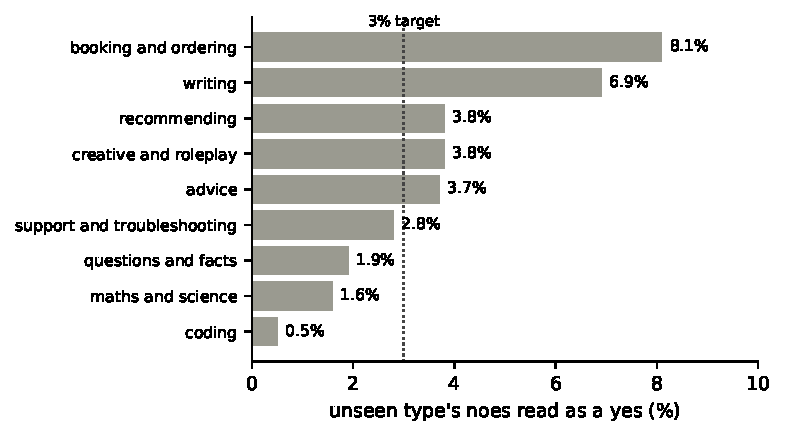
\includegraphics[width=0.75\linewidth]{figures/fig8b_v2_unseen_tasks}
\caption{Sense v2 trained nine more times, each time without one task type and tested on it: the share of that type's noes it read as a yes (leave-one-task-out builds)}
\label{fig:8b}
\end{figure}

\textbf{Sense v3: two questions.} It replaces v2's single question with two, so that thanks for the effort can be told from approval of the result. First, is the reaction a clear verdict on the result at all? Thanks for trying, sarcasm, hedging, settling, silence and moving on without a word are not. Only if it is: which score? The teacher answered both, under a revised guide, for 63,248 reactions: up to 2,000 for each pairing of task type and v2 answer, the eight written kinds again, and 1,778 new reactions of a ninth kind, warm thanks for the effort after a failure. It judged 41\% of them not clear. The teacher is not a perfect reader either (Fig.~\ref{fig:8a}): of the reactions it wrote itself, it read half of the politely unhappy and half of the sarcastic ones as a yes, a quarter of the settling ones, and 16\% of the warm thanks for trying. The student inherits these mistakes; the first question and the thresholds below are what is meant to keep them out of the creature's lessons. One LoRA learns both answers from 44,746 of them, the score weighted by how clear the teacher found the reaction. Its two thresholds, 0.80 for a clear verdict and 0.70 for the score, were chosen on 2,000 held-out reactions as the pair that keeps false accepts, now also counting an unclear reaction read as a yes, at 3\% while keeping the most real yeses. On those reactions it kept 44\% of the teacher's yeses and agreed with the teacher's side on 95\% of the verdicts it gave. In use, a reaction must pass both gates before the creature learns from it (Fig.~\ref{fig:9}). The first gate changes how some common reactions are read (Table~\ref{tab:4}): v2's guide scored moving on to the next request without a word as an 80, a half-weight yes (in use, v2 mostly read it as unclear), and thanks for trying could pass as approval; for v3, neither is a clear verdict.

\begin{figure}[htbp]
\centering
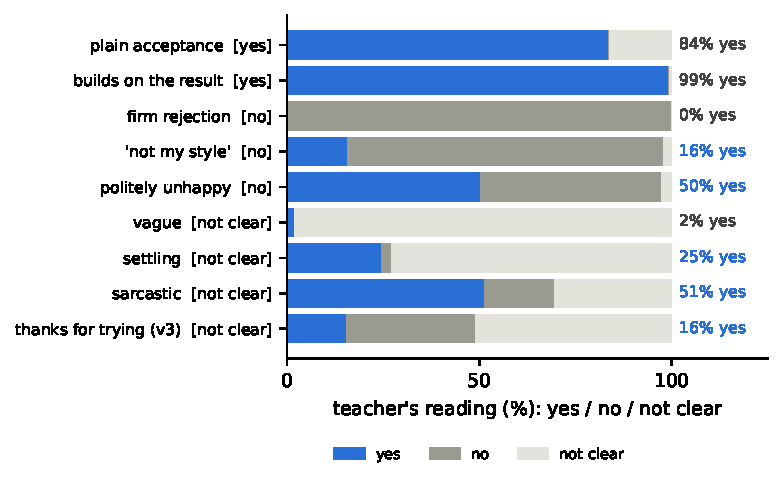
\includegraphics[width=0.75\linewidth]{figures/fig8a_teacher_written}
\caption{How the teacher, under v3's guide, read the 6,506 reactions it wrote; in brackets, the reading each kind was written to have}
\label{fig:8a}
\end{figure}

\begin{figure}[htbp]
\centering
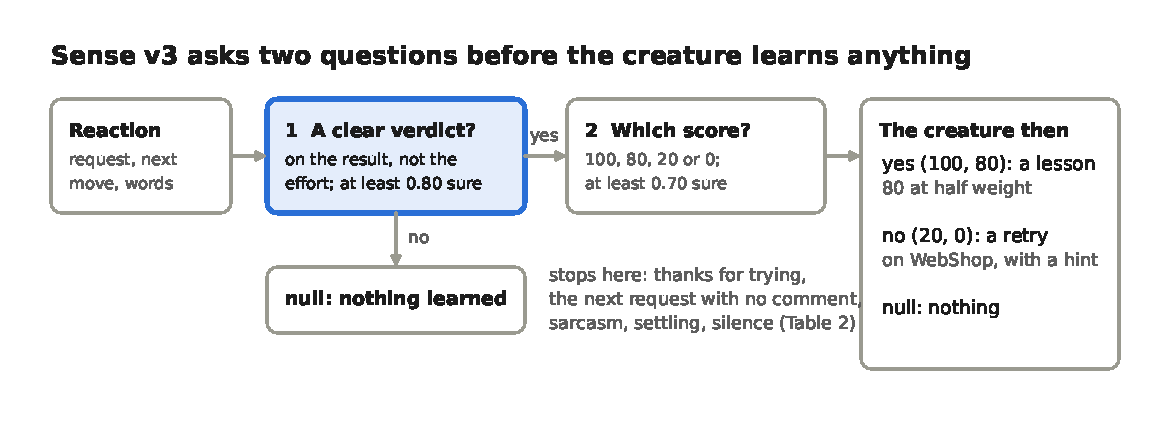
\includegraphics[width=1.0\linewidth]{figures/fig9_sense_decision}
\caption{How sense v3 decides: a reaction must pass both gates before the creature learns from it. v1 and v2 ask only the second question, with one threshold (0.70 and 0.65)}
\label{fig:9}
\end{figure}
